\section{Introduction}\label{sec:intro}

As datacenter links scale to 100--400~Gbps, the receive path between the network interface card (NIC) and the host CPU has become a primary determinant of server efficiency and tail latency~\cite{cai2021hoststack,vuppalapati2024hostnet}. To avoid slow DRAM round trips on every arriving packet, modern server processors use direct cache injection such as Intel Data Direct I/O (DDIO)~\cite{intelddio,huggahalli2005dca}, steering inbound PCIe writes straight into the host last-level cache (LLC). In principle, DDIO lets host cores consume packets at L3 speed without touching main memory.

In practice, DDIO allocates only a small slice of the shared LLC to I/O, typically two cache ways~\cite{farshin2020ddio} (8~MiB out of 60~MiB on our Xeon server). Whenever an incast burst or brief host scheduling pause pushes more packets into host memory than that slice can hold, incoming DMA overwrites unread buffers and forces premature writebacks to DRAM---a pathology known as \emph{Leaky DMA}~\cite{tootoonchian2018resq,farshin2020ddio}. On our testbed, absorbing a 128~MiB receive burst in a conventional host ring drops DDIO hit rate to 16.3\%, raises host LLC read misses to 91.2\%, generates 1.90 host DRAM lines per packet, and inflates the $p99$ lookup latency of a co-located 32~MiB in-memory key-value (KV) store by 3.7--6.3$\times$ (from 41~ns to 153--259~ns; $p999$ reaches 289--315~ns). Even replacing the monotonic host ring with an ideal LIFO buffer pool saves only bursts up to 4~MiB; at 16--128~MiB, co-located KV $p99$ still climbs to 97--205~ns ($p999$ 287--293~ns).

\begin{figure}[t]
  \centering
  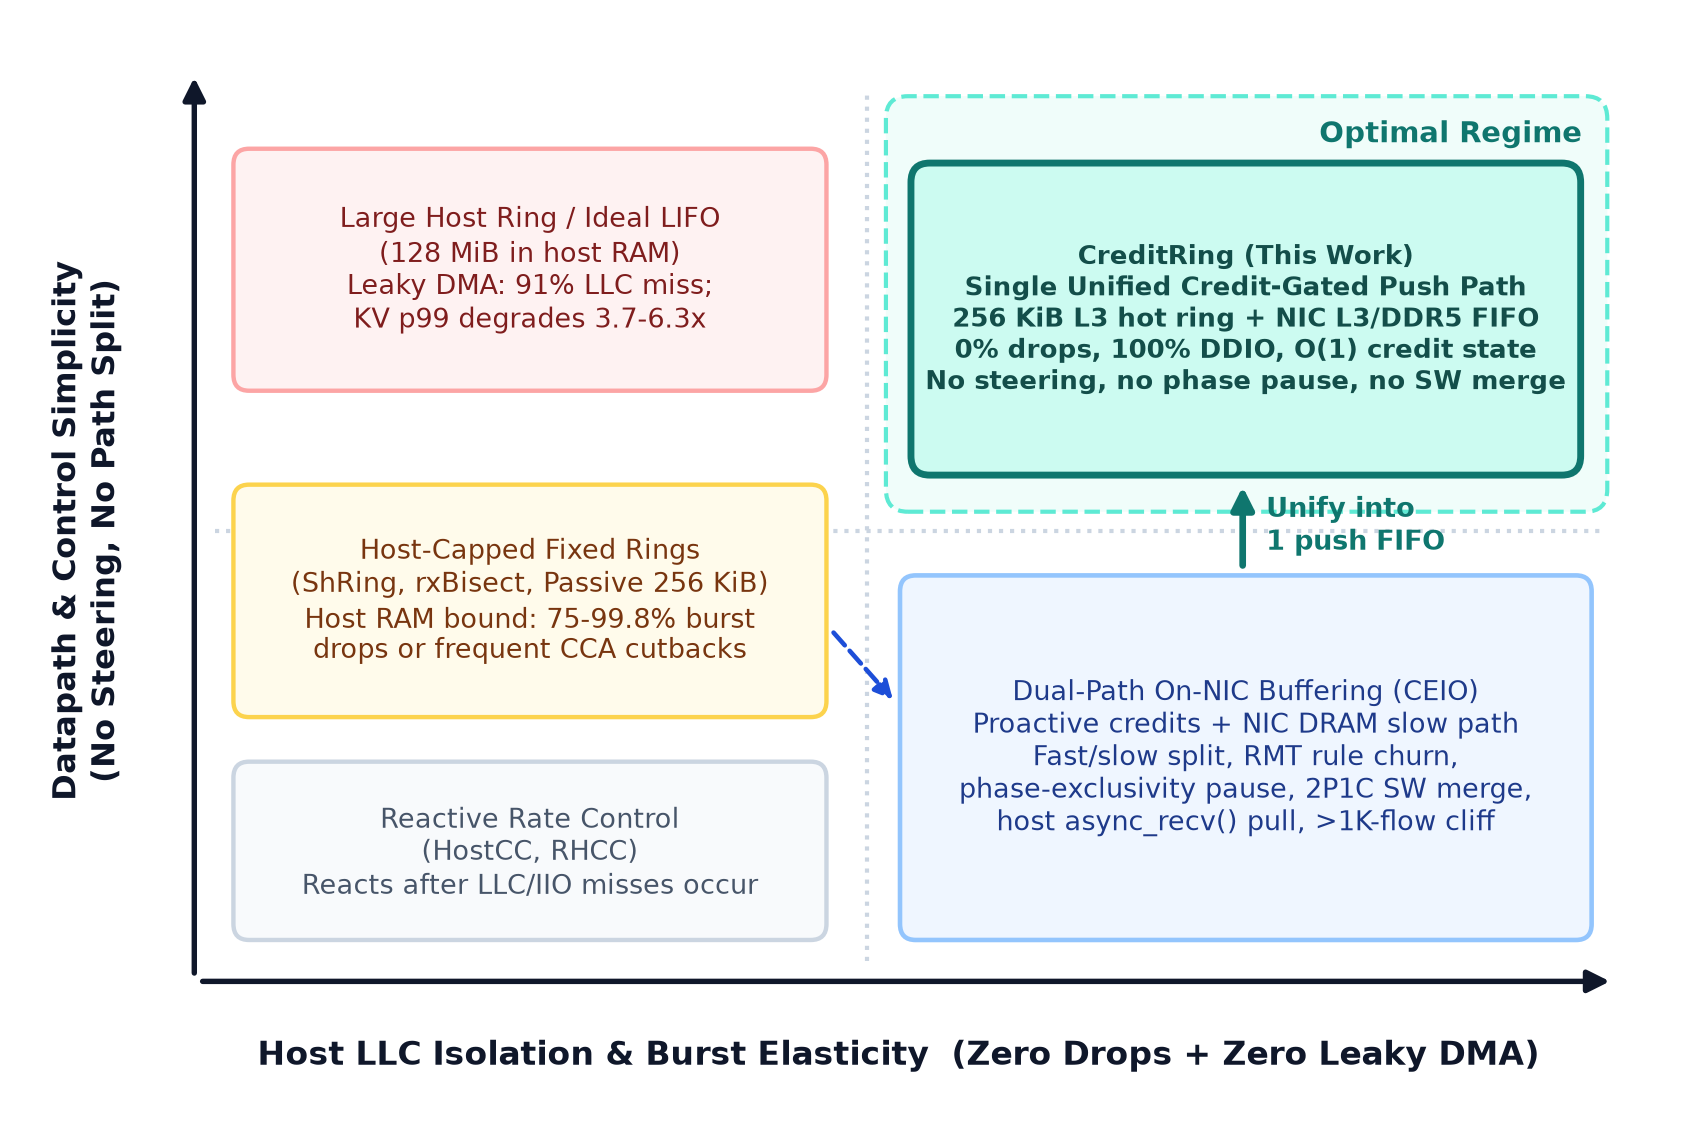
\includegraphics[width=0.95\columnwidth]{figures/fig1_design_space.png}
  \caption{Design space of cache-efficient NIC-to-CPU receive paths. \sys{} reaches the upper-right regime by unifying credit-gated push onto a single L3-pinned host FIFO.}
  \label{fig:design-space}
\end{figure}

Prior systems navigate this tension along three axes, summarized in Figure~\ref{fig:design-space}. \emph{Reactive intra-host congestion control} (HostCC~\cite{agarwal2023hostcc}, RHCC~\cite{wan2025rhcc}) detects IIO or LLC pressure and signals network congestion control, but reacts only after cache misses have started. \emph{Host-capped receive rings} (ShRing~\cite{pismenny2023shring}, rxBisect~\cite{pismenny2025rxbisect}) shrink the receive footprint to stay inside the LLC, yet remain constrained by host memory conservation: once a burst exceeds the small host ring, a passive NIC must either drop packets (75.0--99.8\% loss on a passive 256~KiB ring under 1--128~MiB bursts) or throttle upstream senders. Most recently, \ceio{}~\cite{liu2025ceio} demonstrated that placing proactive credit control and elastic burst buffering on a SmartNIC avoids both misses and drops.

However, \ceio{} preserves the legacy passive DMA ring as a ``fast path'' and grafts on-NIC DRAM buffering onto it as a separate ``slow path.'' That dual-path split introduces five tightly coupled mechanisms: per-flow match-action (RMT) steering rules dynamically rewritten between host LLC and NIC DRAM; a separate slow-path ring in NIC memory; \emph{phase exclusivity} that pauses fast-path DMA while draining slow-path packets so delivery stays ordered without sorting; a two-producer software merge ring (\texttt{SW ring}) in the host driver uniting both hardware rings; and an asynchronous host-initiated DMA pull API (\texttt{async\_recv()}) to fetch buffered packets back across PCIe. Under rapid flow churn (100--500~$\mu$s slots beyond 1,000 flows), per-flow rule management saturates and forces traffic onto the slow path, while even fast-path control adds 10--48\% latency overhead~\cite{liu2025ceio}.

We ask a simpler architectural question: \emph{if the NIC already manages credits and on-NIC burst memory, why maintain two receive paths at all?}

We answer this question with \sys{}, a unified credit-gated receive architecture built around an active NIC. Instead of switching flows between a host fast path and a NIC slow path, \sys{} exposes only a single tiny, strictly L3-pinned receive ring in host memory---\textbf{256~KiB} (4,096 cache-line cells)---for the core credit-gated receive path, and extends the same compact credit discipline to native NIC DMA receive rings ($\le$2~MiB total across four lanes) for large 1--4~KiB Ethernet frames. Every arriving packet enters the same FIFO queue on the NIC. When credits are available, the NIC pushes the packet immediately across PCIe into the host hot ring; when credits are exhausted, the packet waits in the NIC's own memory hierarchy (\textbf{48~MiB on-NIC L3} backed by \textbf{6-channel on-NIC DDR5}) and is pushed through the exact same host ring as the host returns batched \texttt{TAKEN} credits via a single posted MMIO write.

This single architectural unification eliminates path switching, RMT flow-table rewrites, phase-exclusivity pauses, dual-ring software merges, host-initiated DMA pulls, and per-flow scaling cliffs by construction. Credit enforcement reduces to an $O(1)$ integer comparison on a NIC-local cached counter per host receive ring, completely independent of the number of active network flows.

We implement \sys{} in Rust on an unmodified PCIe Gen5 Intel Xeon server (with full hardware IOMMU enabled) paired with a Marvell OCTEON~10 CN106 100GbE SmartNIC and a second physical 100GbE peer. Rather than evaluating against an untuned stock driver, we also engineer a heavily optimized asynchronous descriptor-ring baseline (\texttt{SDP fair-full}) via single-variable ablation (eliminating synchronous tail waits and fitting its receive ring inside DDIO to reach 100.0\% DDIO and 76$\times$ fewer host DRAM writes than the non-DDIO-sized ring). Across 1,089 verified zero-error hardware runs with 100\% non-multiplexed host and NIC performance counters, we make four contributions:

\begin{enumerate}
  \item \textbf{Unified push-only credit ring (\S\ref{sec:overview}--\S\ref{sec:design}):} We formulate \sys{}'s single-FIFO credit protocol over a 256~KiB L3-pinned host ring, prove its overflow-free, ordered, and deadlock-free invariants, and extend the same compact credit discipline to $\le$2~MiB DMA receive rings for 1--4~KiB frames.
  \item \textbf{Zero-backlog overhead and DRAM offload duality (\S\ref{sec:eval-burst}):} Credit checks add \textbf{+6~ns} to $W{=}1$ RTT (0.887 $\to$ 0.893~$\mu$s) with zero $W{=}32$ throughput loss. Across 64~KiB--128~MiB bursts, \sys{} locks DDIO at \textbf{100.0\%} and LLC misses at \textbf{0.01\%}, cuts host DRAM traffic by \textbf{98.9\%} (971.5 $\to$ 10.7~MiB), eliminates system-wide DRAM for bursts $\le$32~MiB inside NIC L3, offloads $>$48~MiB bursts onto NIC DDR5, and holds a flat \textbf{0.905~$\mu$s} ($p99$ 0.945~$\mu$s) refill hop.
  \item \textbf{Co-located KV isolation and refill wire wall (\S\ref{sec:eval-kv}):} Across 1--128~MiB bursts, \sys{} is the only scheme achieving \textbf{0.0\% drops} and untouched 32~MiB KV tail latency (\textbf{41--42~ns} $p99$, 43--47~ns $p999$), versus 3.7--6.3$\times$ $p99$ degradation on monotonic rings, up to 5.0$\times$ on LIFO pools, and 75.0--99.8\% drops on passive 256~KiB rings. We also show that 1, 2, and 4 NIC refill cores converge at \textbf{177.2--177.3~M/s} (\textbf{99.1\%} of the 179.0~M/s PCIe Gen5 $\times$4 64~B TLP wall), fixing the drain crossover at 32--48~MiB (+12.6\% faster at 64~MiB).
  \item \textbf{Single-core 100GbE RX and end-to-end DirectPush RPC/KV (\S\ref{sec:eval-rx}--\S\ref{sec:eval-rpc}):} Integrated into our end-to-end push/DMA datapath (\emph{DirectPush}, combining \sys{} on RX with \texttt{MOVDIR64B} host-to-NIC TX, native \texttt{DPI DMA} for $\ge$1~KiB payloads, and zero-atomic NIC ingress), one 3.90~GHz host core saturates 100GbE RX at 110~B (96.2~Mpps), 134~B (80.9~Mpps), 1094~B, and 4096~B with zero C2H drops and 22.5$\times$ less host DRAM than 2048-descriptor SDP. On a dual-host 100GbE 32.5~MiB KV server against tuned 4-queue async SDP, this integrated datapath raises saturation throughput up to \textbf{+55\%} (64~B) and \textbf{+16\%} (mixed), cuts open-loop $p99$ by \textbf{63.5\%} (64~B) and \textbf{49.7\%} (mixed small), and saves \textbf{15.2--42.4\%} net CPU and \textbf{17.2--62.5\%} bidirectional PCIe bytes. A companion TX check confirms expanding the host's retained reply pool from 4~MiB to 128~MiB causes a \textbf{92--98$\times$ DRAM surge} and 14--38\% throughput loss.
\end{enumerate}
